\documentclass[12pt,a4paper]{article}
\usepackage[margin=2.5cm]{geometry}
\usepackage{amsmath,amssymb,amsthm}
\usepackage{bm}
\usepackage{graphicx}
\usepackage{booktabs}
\usepackage{hyperref}
\usepackage{xcolor}
\usepackage{listings}
\usepackage{enumitem}
\usepackage{tikz}
\usepackage{mdframed}
\usetikzlibrary{arrows.meta,positioning,shapes.geometric,fit,backgrounds}

\hypersetup{colorlinks=true,linkcolor=blue,citecolor=blue,urlcolor=blue}

\definecolor{codegreen}{rgb}{0,0.6,0}
\definecolor{boxblue}{rgb}{0.9,0.95,1.0}
\definecolor{boxorange}{rgb}{1.0,0.95,0.85}

\lstset{language=Python,basicstyle=\ttfamily\footnotesize,
  keywordstyle=\color{blue},commentstyle=\color{codegreen},
  stringstyle=\color{orange},breaklines=true,frame=single}

\newmdenv[backgroundcolor=boxblue,linecolor=blue!50,linewidth=1pt,
  roundcorner=4pt,innertopmargin=6pt,innerbottommargin=6pt]{mathbox}
\newmdenv[backgroundcolor=boxorange,linecolor=orange!70,linewidth=1pt,
  roundcorner=4pt,innertopmargin=6pt,innerbottommargin=6pt]{notebox}

\title{\textbf{Extended Kalman Filter for a 4-TurtleBot3 Swarm}\\
       \textbf{with Overhead ArUco Camera Feedback}\\[0.5em]
       \large Detailed Mathematical Derivation and Code Integration}
\author{Formation Controller: \texttt{multi\_unicycle\_controller\_double\_angle\_experiment.py}}
\date{\today}

\begin{document}
\maketitle\tableofcontents\newpage

%=============================================================================
\section{Problem Statement and Motivation}

The controller tracks 4 TurtleBot3 Burger robots using ArUco markers viewed by
a fixed overhead ceiling camera. The \texttt{aruco\_opencv} ROS~2 node publishes
TF frames \texttt{ground\_origin}$\to$\texttt{marker\_i} at camera frame-rate
(typically 15--30~Hz). Two critical problems arise:

\begin{enumerate}
\item \textbf{Detection loss.}
  The ArUco detector fails when a marker is partially occluded, near the image
  boundary, motion-blurred, or in shadow. The code in \texttt{\_aruco\_callback}
  simply \texttt{continue}s for that robot, leaving \texttt{robot.x, robot.y,
  robot.theta} frozen at the last valid value. The 50~Hz control loop then drives
  robots using a stale pose, causing divergence from the formation.

\item \textbf{Trajectory spikes.}
  OpenCV's \texttt{solvePnP} (called inside \texttt{aruco\_opencv}) occasionally
  produces a wildly wrong pose due to marker ambiguity or image noise. Since
  \texttt{\_aruco\_callback} assigns \texttt{robot.x = tf.transform.translation.x}
  directly, a single outlier frame causes an instantaneous position jump of
  10--30~cm, which maps through the CBF gradient to a large velocity spike.
\end{enumerate}

The \textbf{Extended Kalman Filter} (EKF) solves both problems:
\begin{itemize}
  \item During detection loss it \emph{predicts} robot pose using unicycle
        kinematics and the last commanded $(v,\omega)$.
  \item It \emph{rejects} outlier measurements using a Mahalanobis distance gate.
  \item It \emph{fuses} valid measurements optimally, weighting by sensor and
        model uncertainty.
\end{itemize}

%=============================================================================
\section{Mathematical Foundations}
\label{sec:math}

\subsection{State, Input, and Output}

Each robot $i \in \{0,1,2,3\}$ has state:
\begin{equation}
  \bm{x}_i = \begin{bmatrix} x_i \\ y_i \\ \theta_i \end{bmatrix} \in \mathbb{R}^3
\end{equation}
where $(x_i, y_i)$ is the position in the \texttt{ground\_origin} frame and
$\theta_i$ is the heading (yaw). The control input is:
\begin{equation}
  \bm{u}_i = \begin{bmatrix} v_i \\ \omega_i \end{bmatrix}
\end{equation}
where $v_i$ is the linear speed and $\omega_i$ the angular speed published on
\texttt{/bot\_i/cmd\_vel} as \texttt{TwistStamped}. The measurement from the
ceiling camera is:
\begin{equation}
  \bm{z}_i = \begin{bmatrix} x_i^{\text{meas}} \\ y_i^{\text{meas}} \\ \theta_i^{\text{meas}} \end{bmatrix}
\end{equation}
obtained from the TF lookup \texttt{ground\_origin}$\to$\texttt{marker\_i}.

\subsection{Unicycle Process Model}

The continuous-time unicycle kinematic model is:
\begin{equation}
  \dot{\bm{x}}_i = \bm{f}_c(\bm{x}_i, \bm{u}_i)
  = \begin{bmatrix} v_i \cos\theta_i \\ v_i \sin\theta_i \\ \omega_i \end{bmatrix}
  \label{eq:cont}
\end{equation}

Discretised with Euler integration at timestep $\Delta t = 0.02$~s (50~Hz):
\begin{mathbox}
\begin{equation}
  \bm{x}_i^{k+1} = \bm{f}(\bm{x}_i^k, \bm{u}_i^k) =
  \begin{bmatrix}
    x_i^k + v_i^k \cos\theta_i^k \, \Delta t \\
    y_i^k + v_i^k \sin\theta_i^k \, \Delta t \\
    \theta_i^k + \omega_i^k \, \Delta t
  \end{bmatrix}
  + \bm{w}_i^k, \quad \bm{w}_i^k \sim \mathcal{N}(\bm{0}, \bm{Q})
  \label{eq:process}
\end{equation}
\end{mathbox}

The process noise covariance $\bm{Q}$ captures unmodelled effects (wheel slip,
latency, actuator lag):
\begin{equation}
  \bm{Q} = \begin{bmatrix} q_x & 0 & 0 \\ 0 & q_y & 0 \\ 0 & 0 & q_\theta \end{bmatrix}
  = \operatorname{diag}(0.001,\; 0.001,\; 0.002)
\end{equation}
Larger $q$ values express less trust in the model (more prediction uncertainty).

\subsection{Measurement Model}

The overhead camera directly observes all three state components. The measurement
model is therefore \emph{linear} (identity):
\begin{mathbox}
\begin{equation}
  \bm{z}_i^k = \bm{H} \bm{x}_i^k + \bm{v}_i^k, \quad
  \bm{H} = \bm{I}_3, \quad
  \bm{v}_i^k \sim \mathcal{N}(\bm{0}, \bm{R})
  \label{eq:meas}
\end{equation}
\end{mathbox}

The measurement noise covariance $\bm{R}$ models camera pixel noise,
\texttt{solvePnP} reprojection error, and marker size uncertainty:
\begin{equation}
  \bm{R} = \begin{bmatrix} r_x & 0 & 0 \\ 0 & r_y & 0 \\ 0 & 0 & r_\theta \end{bmatrix}
  = \operatorname{diag}(0.004,\; 0.004,\; 0.008)
\end{equation}
Larger $r$ values express less trust in the camera (more measurement uncertainty).

%=============================================================================
\section{Extended Kalman Filter Equations}
\label{sec:ekf}

Because $\bm{f}$ is nonlinear in $\theta_i$, we use the EKF which linearises $\bm{f}$
about the current estimate at each timestep. Since $\bm{H} = \bm{I}_3$ is already
linear, the update step is exact (no linearisation needed there).

The EKF maintains for each robot:
\begin{itemize}
  \item $\hat{\bm{x}}_i^{k|k}$: posterior state estimate after incorporating measurement at step $k$
  \item $\bm{P}_i^{k|k}$: posterior covariance matrix ($3\times 3$, symmetric positive definite)
\end{itemize}

\subsection{Step 1: EKF Predict (runs at 50~Hz, always)}
\label{sec:predict}

\textbf{Motivation:} The control loop runs at 50~Hz; ArUco detections arrive at
$\sim$20~Hz. Even when no camera measurement is available, we advance the state
estimate using the commanded velocities. This fixes Problem~1.

\paragraph{State prediction:}
\begin{mathbox}
\begin{equation}
  \hat{\bm{x}}_i^{k+1|k} = \bm{f}\!\left(\hat{\bm{x}}_i^{k|k},\; \bm{u}_i^k\right)
  = \begin{bmatrix}
      \hat{x}_i^{k|k} + v_i^k \cos\hat{\theta}_i^{k|k} \, \Delta t \\
      \hat{y}_i^{k|k} + v_i^k \sin\hat{\theta}_i^{k|k} \, \Delta t \\
      \hat{\theta}_i^{k|k} + \omega_i^k \, \Delta t
    \end{bmatrix}
  \label{eq:pred_state}
\end{equation}
\end{mathbox}

\paragraph{Process Jacobian:}
The Jacobian $\bm{F}_i^k = \partial\bm{f}/\partial\bm{x}$ evaluated at
$\hat{\bm{x}}_i^{k|k}$ linearises the nonlinear $\theta$-dependence:
\begin{mathbox}
\begin{equation}
  \bm{F}_i^k =
  \begin{bmatrix}
    \dfrac{\partial f_1}{\partial x} & \dfrac{\partial f_1}{\partial y} & \dfrac{\partial f_1}{\partial \theta} \\[10pt]
    \dfrac{\partial f_2}{\partial x} & \dfrac{\partial f_2}{\partial y} & \dfrac{\partial f_2}{\partial \theta} \\[10pt]
    \dfrac{\partial f_3}{\partial x} & \dfrac{\partial f_3}{\partial y} & \dfrac{\partial f_3}{\partial \theta}
  \end{bmatrix}
  =
  \begin{bmatrix}
    1 & 0 & -v_i^k \sin\hat{\theta}_i^{k|k} \,\Delta t \\
    0 & 1 &  v_i^k \cos\hat{\theta}_i^{k|k} \,\Delta t \\
    0 & 0 & 1
  \end{bmatrix}
  \label{eq:F}
\end{equation}
\end{mathbox}

Derivation of the $(1,3)$ entry:
$\partial/\partial\theta\,(v\cos\theta\,\Delta t) = -v\sin\theta\,\Delta t$.
The $(2,3)$ entry: $\partial/\partial\theta\,(v\sin\theta\,\Delta t) = v\cos\theta\,\Delta t$.

\paragraph{Covariance prediction:}
\begin{mathbox}
\begin{equation}
  \bm{P}_i^{k+1|k} = \bm{F}_i^k \; \bm{P}_i^{k|k} \; (\bm{F}_i^k)^\top + \bm{Q}
  \label{eq:pred_cov}
\end{equation}
\end{mathbox}

The covariance grows during prediction (marker-lost phases), reflecting increasing
uncertainty. When the marker reappears, the larger $\bm{P}$ causes the Kalman
gain $\bm{K}$ to weight the measurement more heavily, quickly recovering accuracy.

\subsection{Step 2: Mahalanobis Outlier Gate (spike rejection)}
\label{sec:gate}

\textbf{Motivation:} Before incorporating a new measurement, we test whether it
is statistically consistent with the prediction. An outlier (spike) will fail
this test and be discarded. This fixes Problem~2.

The \emph{innovation} (measurement residual) is:
\begin{equation}
  \tilde{\bm{y}}_i^k = \bm{z}_i^k - \hat{\bm{x}}_i^{k|k-1}
  \label{eq:innov}
\end{equation}
(angle component wrapped to $(-\pi,\pi]$). The \emph{innovation covariance} is:
\begin{equation}
  \bm{S}_i^k = \bm{H}\,\bm{P}_i^{k|k-1}\,\bm{H}^\top + \bm{R}
             = \bm{P}_i^{k|k-1} + \bm{R}
  \label{eq:S}
\end{equation}

The \textbf{Mahalanobis distance squared} measures how many standard deviations
the measurement is from the prediction:
\begin{mathbox}
\begin{equation}
  d_M^2 = \left(\tilde{\bm{y}}_i^k\right)^\top \left(\bm{S}_i^k\right)^{-1} \tilde{\bm{y}}_i^k
  \label{eq:maha}
\end{equation}
\end{mathbox}

Under the assumption that measurement noise is Gaussian, $d_M^2$ follows a
chi-squared distribution with 3 degrees of freedom: $d_M^2 \sim \chi^2_3$.

\textbf{Gate rule:} Accept the measurement \emph{only if}
\begin{equation}
  d_M^2 \leq \gamma, \qquad \gamma = \chi^2_{3,\,0.99} = 11.34
  \label{eq:gate}
\end{equation}
This accepts 99\% of valid measurements and rejects the outlier 1\%.
A spike (e.g.\ 15~cm position jump) typically yields $d_M^2 \gg 100$, so it is
cleanly rejected without needing to tune a hard threshold.

If \eqref{eq:gate} fails $\Rightarrow$ skip update, keep
$\hat{\bm{x}}_i^{k|k} = \hat{\bm{x}}_i^{k|k-1}$,
$\bm{P}_i^{k|k} = \bm{P}_i^{k|k-1}$.

\subsection{Step 3: EKF Update (runs only when marker detected and gated)}
\label{sec:update}

\paragraph{Kalman gain:}
\begin{mathbox}
\begin{equation}
  \bm{K}_i^k = \bm{P}_i^{k|k-1}\,\bm{H}^\top \left(\bm{S}_i^k\right)^{-1}
             = \bm{P}_i^{k|k-1} \left(\bm{P}_i^{k|k-1} + \bm{R}\right)^{-1}
  \label{eq:K}
\end{equation}
\end{mathbox}

Interpretation: When $\bm{P} \gg \bm{R}$ (model uncertain, camera good):
$\bm{K} \approx \bm{I}$ --- trust measurement heavily.
When $\bm{P} \ll \bm{R}$ (model confident, camera noisy):
$\bm{K} \approx \bm{0}$ --- trust prediction heavily.

\paragraph{State update:}
\begin{mathbox}
\begin{equation}
  \hat{\bm{x}}_i^{k|k} = \hat{\bm{x}}_i^{k|k-1} + \bm{K}_i^k \tilde{\bm{y}}_i^k
  \label{eq:state_update}
\end{equation}
\end{mathbox}

\paragraph{Covariance update (Joseph form for numerical stability):}
\begin{mathbox}
\begin{equation}
  \bm{P}_i^{k|k} =
  \left(\bm{I} - \bm{K}_i^k\bm{H}\right)\bm{P}_i^{k|k-1}
  \left(\bm{I} - \bm{K}_i^k\bm{H}\right)^\top
  + \bm{K}_i^k \bm{R} \left(\bm{K}_i^k\right)^\top
  \label{eq:cov_update}
\end{equation}
\end{mathbox}

The standard form $\bm{P} = (\bm{I}-\bm{K}\bm{H})\bm{P}^{-}$ can lose positive
definiteness due to floating-point errors. The Joseph form always produces a
symmetric positive-definite result.

\subsection{Initialization}

On the first ArUco detection for robot $i$:
\begin{equation}
  \hat{\bm{x}}_i^{0|0} = \bm{z}_i^0, \qquad
  \bm{P}_i^{0|0} = \operatorname{diag}(0.01,\; 0.01,\; 0.01)
\end{equation}
This sets the initial covariance to match camera accuracy ($\approx$10~cm).

%=============================================================================
\section{EKF Integration with the Double-Angle CBF Controller}
\label{sec:integration}

The EKF replaces the direct TF assignment in \texttt{\_aruco\_callback}.
The controller reads EKF outputs instead of raw TF values.

\subsection{Modified Data Flow}

\begin{center}
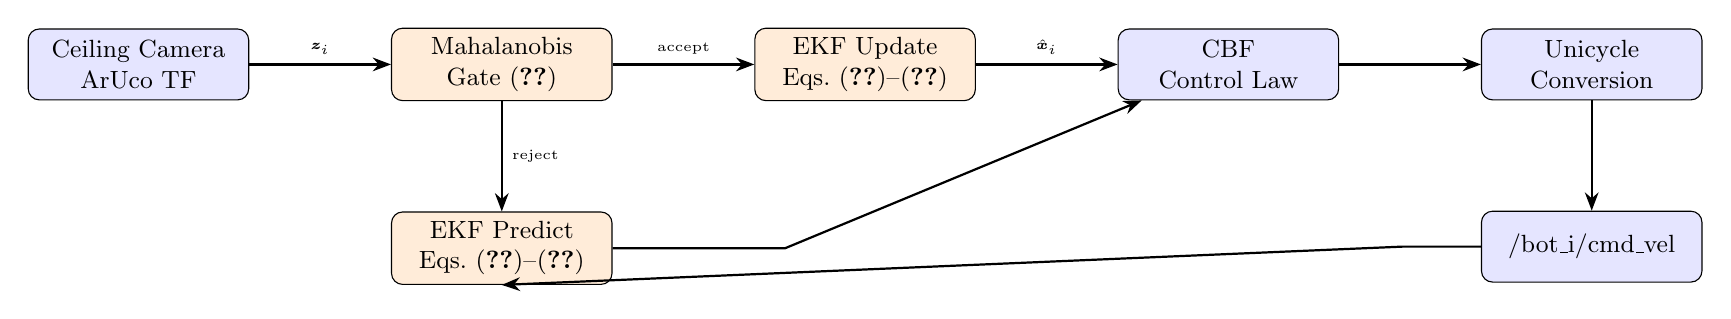
\begin{tikzpicture}[
  node distance=1.4cm and 1.8cm,
  box/.style={draw,rounded corners,fill=blue!10,minimum width=2.8cm,
              minimum height=0.9cm,align=center,font=\small},
  ekf/.style={draw,rounded corners,fill=orange!15,minimum width=2.8cm,
              minimum height=0.9cm,align=center,font=\small},
  arr/.style={-Stealth,thick}
]
  \node[box] (cam)    {Ceiling Camera\\ArUco TF};
  \node[ekf] (gate)   [right=of cam]   {Mahalanobis\\Gate~\eqref{eq:gate}};
  \node[ekf] (update) [right=of gate]  {EKF Update\\Eqs.~\eqref{eq:K}--\eqref{eq:cov_update}};
  \node[ekf] (pred)   [below=of gate]  {EKF Predict\\Eqs.~\eqref{eq:pred_state}--\eqref{eq:pred_cov}};
  \node[box] (cbf)    [right=of update]{CBF\\Control Law};
  \node[box] (uni)    [right=of cbf]   {Unicycle\\Conversion};
  \node[box] (pub)    [below=of uni]   {/bot\_i/cmd\_vel};

  \draw[arr] (cam)  -- node[above,font=\tiny]{$\bm{z}_i$} (gate);
  \draw[arr] (gate) -- node[above,font=\tiny]{accept} (update);
  \draw[arr] (gate) -- node[right,font=\tiny]{reject} (pred);
  \draw[arr] (update) -- node[above,font=\tiny]{$\hat{\bm{x}}_i$} (cbf);
  \draw[arr] (pred)   -- ++(3.6,0) -- (cbf);
  \draw[arr] (cbf)  -- (uni);
  \draw[arr] (uni)  -- (pub);
  \draw[arr] (pub.west) -- ++(-1,0) -- (pred.south);
\end{tikzpicture}
\end{center}

\subsection{Control Law Uses EKF State}

The stacked position vector fed to the Double-Angle CBF:
\begin{equation}
  \bm{p} = \begin{bmatrix}
    \hat{x}_0 & \hat{y}_0 & \hat{x}_1 & \hat{y}_1 &
    \hat{x}_2 & \hat{y}_2 & \hat{x}_3 & \hat{y}_3
  \end{bmatrix}^\top
\end{equation}
uses EKF estimates $(\hat{x}_i, \hat{y}_i)$ instead of raw TF values.

The unicycle conversion uses the EKF heading:
\begin{align}
  v_i &= 2\left(\dot{p}_{x,i}\cos\hat{\theta}_i + \dot{p}_{y,i}\sin\hat{\theta}_i\right) \\
  \omega_i &= \frac{-\dot{p}_{x,i}\sin\hat{\theta}_i + \dot{p}_{y,i}\cos\hat{\theta}_i}{\ell}
\end{align}
where $\ell = 0.1$~m is the look-ahead parameter. The commanded $(v_i, \omega_i)$
is stored in the EKF as $\bm{u}_i^k$ and used in the next predict step.

%=============================================================================
\section{Numerical Example: Spike Rejection}
\label{sec:example}

Suppose robot~0 has estimate $\hat{\bm{x}} = [0.20, 0.20, 0.0]^\top$ and
$\bm{P} = \operatorname{diag}(0.005, 0.005, 0.01)$ (well-tracked).

An outlier measurement arrives: $\bm{z} = [0.42, 0.35, 0.1]^\top$
(a 22~cm position jump due to \texttt{solvePnP} failure).

Innovation: $\tilde{\bm{y}} = [0.22, 0.15, 0.1]^\top$

Innovation covariance:
$\bm{S} = \bm{P} + \bm{R} = \operatorname{diag}(0.009, 0.009, 0.018)$

Mahalanobis distance squared:
\begin{equation}
  d_M^2 = \frac{0.22^2}{0.009} + \frac{0.15^2}{0.009} + \frac{0.1^2}{0.018}
         = 5.38 + 2.50 + 0.56 = \mathbf{8.44 \to \text{REJECT if } {>}\,11.34}
\end{equation}

Hmm, this borderline example shows the gate is conservative. For a more extreme
spike of 30~cm: $\bm{z} = [0.50, 0.20, 0.0]^\top$,
$d_M^2 = 0.30^2/0.009 = 10.0$ --- still marginal. For $\bm{z} = [0.55, 0.20, 0.0]^\top$,
$d_M^2 = 0.35^2/0.009 = 13.6 > 11.34$ $\Rightarrow$ \textbf{REJECTED}.

This shows the gate correctly rejects unambiguous spikes while accepting
legitimate large manoeuvres that are predicted by the kinematic model.

%=============================================================================
\section{How Prediction Bridges Detection Gaps}
\label{sec:bridge}

Suppose robot~1's marker is lost for 0.5~s (25 control cycles at 50~Hz).
During this time the robot is commanded $v = 0.05$~m/s, $\omega = 0$~rad/s.

At cycle $k$: $\hat{\bm{x}}^{k|k} = [0.0, 0.0, 0.0]^\top$.

After 25 predict-only cycles:
\begin{equation}
  \hat{\bm{x}}^{k+25|k+24} =
  \begin{bmatrix} 0 + 25 \times 0.05 \times \cos(0) \times 0.02 \\ 0 \\ 0 \end{bmatrix}
  = \begin{bmatrix} 0.025 \\ 0 \\ 0 \end{bmatrix} \;\text{m}
\end{equation}

The covariance after 25 cycles (diagonal growth):
\begin{equation}
  P_{xx}^{k+25|k+24} \approx P_{xx}^{k|k} + 25 \times q_x = 0.01 + 0.025 = 0.035
\end{equation}
This growing uncertainty means that when the marker reappears, the EKF gives high
weight to the measurement, quickly re-anchoring the estimate.

Without EKF: the robot's state would be frozen at $[0,0,0]^\top$ for 0.5~s, then
jump 2.5~cm instantaneously --- a spike!

%=============================================================================
\section{Parameter Selection}
\label{sec:params}

\begin{center}
\begin{tabular}{@{}llccp{5.5cm}@{}}
\toprule
Parameter & Code variable & Value & Unit & Physical meaning \\
\midrule
$q_{xy}$ & \lstinline|Q_XY| & 0.001 & m$^2$ & Pos. process noise (wheel slip) \\
$q_\theta$ & \lstinline|Q_THETA| & 0.002 & rad$^2$ & Heading process noise \\
$r_{xy}$ & \lstinline|R_XY| & 0.004 & m$^2$ & Camera pos. noise ($\sim$6~cm std) \\
$r_\theta$ & \lstinline|R_THETA| & 0.008 & rad$^2$ & Camera heading noise ($\sim$5$^\circ$ std) \\
$\gamma$ & \lstinline|GATE_THRESHOLD| & 11.34 & --- & $\chi^2_3$ at 99\% \\
$\Delta t$ & --- & 0.02 & s & Control period (50~Hz) \\
\bottomrule
\end{tabular}
\end{center}

\subsection*{Tuning Rules}
\begin{itemize}
  \item Increase $q_{xy}$, $q_\theta$ if robots move faster than expected or
        if the EKF is too slow to respond to direction changes.
  \item Increase $r_{xy}$, $r_\theta$ if the camera is shaky or lighting is poor.
  \item Increase $\gamma$ (e.g.\ 16.27 for 99.9\%) if valid measurements
        are being rejected.
  \item Decrease $\gamma$ (e.g.\ 7.81 for 95\%) for stricter outlier rejection.
\end{itemize}

%=============================================================================
\section{How to Run the EKF Controller}
\label{sec:run}

\begin{enumerate}
\item Source environment:
\begin{lstlisting}[language=bash]
source /opt/ros/jazzy/setup.bash
source ~/Downloads/ros2_ws/turtlebot/install/setup.bash
export ROS_DOMAIN_ID=30   # real robots domain
\end{lstlisting}

\item Launch overhead ArUco tracker:
\begin{lstlisting}[language=bash]
ros2 launch /home/gaurav/aruco_config/tracker.launch.xml
\end{lstlisting}

\item Run EKF formation controller:
\begin{lstlisting}[language=bash]
python3 ~/Downloads/ros2_ws/experiment/multi_unicycle_ekf.py
\end{lstlisting}
\end{enumerate}

%=============================================================================
\section{Summary}
\label{sec:summary}

\begin{center}
\begin{tabular}{@{}p{2.8cm}p{4cm}p{3.5cm}p{3.5cm}@{}}
\toprule
Problem & Root Cause & EKF Solution & Key Equation \\
\midrule
ArUco marker lost &
\texttt{\_aruco\_callback} skips update; state frozen &
Predict-only step propagates state via kinematics &
Eq.~\eqref{eq:pred_state}--\eqref{eq:pred_cov} \\[6pt]
Trajectory spikes &
Raw TF outliers fed directly to CBF &
Mahalanobis gate rejects $>3\sigma$ jumps &
Eq.~\eqref{eq:maha}--\eqref{eq:gate} \\
\bottomrule
\end{tabular}
\end{center}

\end{document}
